\documentclass{article}
\usepackage[utf8]{inputenc}
\usepackage[margin=1in]{geometry}
\usepackage{graphicx}
\usepackage{natbib}
\usepackage{enumitem}
\usepackage{array}
\usepackage{gensymb}
\usepackage{indentfirst}
\graphicspath{ {Images/} }
\usepackage{float}

\title{Physics 111A Fall 2016- Lab 3\\
Semiconductor Diodes}
\author{Joshua Levy\\Lab Partner: Alex Chuang}
\date{September 16th, 2016}

\begin{document}

\maketitle

\section{Lab Report}
\subsection{Forward and Reverse Diode Behavior}
    $V_{forward} = 0.622 V$.
    $V_{reverse}$, 'OPEN' displayed\\ The forward voltage drop is exactly what we expected, and the 
    'OPEN' signal for the reverse bias measurement conforms to expectations. The diode performs unidirectionally.
\subsection{Forward Voltage Drop Temperature Dependence}
    See signature page.\\
    $V_{forward} = 0.615 V$.
    $V_{forwardSqueeze} = 0.58 V$.
    $V_{forwardNitrogen} = 1.04 V$.
\subsection{Offset Adder Functionality I}
    See Table 1 for data. See Figure 1 for a plot of the data. The figure depicts the measured output voltage versus the measured current for a given load resistance. Of each colored scatter plot represents different load resistances, and as it can be noticed, the curves generated look very stiff. The data points that are left most and right most for each curve were found by turning the offset adjuster to its maximum and minimum setting. However, you can see that the magnitude of the upper and lower currents were at about 24 mA. The data in between is thus very stiff and the slopes of each curve as found from the trend line (converting to proper magnitude units) roughly corresponds to the load resistance.
\subsection{Diode Characteristic Curve}
    Table 2 depicts data describing the generated Diode Characteristic curve I(V), found from recording corresponding measured current values after adjusting the input voltage of the circuit using an offset adjuster. The data has been displayed in a linear plot in Figure 2 and in a log-linear plot in Figure 3. $V_{measured}$ is the voltage found across the diode.
\subsection{Diode Characteristic Curve Measured with the Curve Tracer}
    See signature page.\\ For use with future sections:
    \\\indent For diode at room temperature, $I_{sat}$ measured to be $2.70*10^{-5} mA = 27 nA$, $V_{cof}$, the voltage coefficient, measured to be 19.246 [1/V], and $n_{calculated} = \frac{e}{kTV_{cof}} \approx 2.055$.
    \\\indent For diode at 77K with nitrogen, $I_{sat}$ measured to be $1.58*10^{-37} mA$, $V_{cof}$ measured to be 73.08 [1/V], and $n_{calculated} = \frac{e}{kTV_{cof}} \approx 2.059$. The n-values are constant amongst the two temperatures. Figures 4 and 5 display the characteristic curves of the diodes at room temperature and 77K respectively.
\subsection{Diode Reverse Current}
    The resistor R (10M$\Omega$) to be used was measured to be $\sim 9.73M\Omega$. The voltage measured across R was $V_{meas} = 32 mV$. Because R is being used in parallel to the impedance of the DMM (Z = 10 M$\Omega$), we experience impedance matching, and deduce an equivalent imput impedance when trying to find current:
    \begin{equation}
        Z_{eq} = \frac{RZ}{R+Z}
    \end{equation}
    Thus the current measured is:
    \begin{equation}
        I = \frac{V_{meas}}{Z_{eq}} = \frac{V_{meas}(R+Z)}{RZ} = \frac{32mV*(9.73 + 10)M\Omega}{9.73M\Omega*10M\Omega} \approx 6.489 nA
    \end{equation}
    This is at a similar order of magnitude as the magnitude of $I_{sat}$ found in the previous section (27 nA). $I_{sat}$ in the previous section is about 4 to 5 times larger than the $I$ found in this section, which means that they are at comparable orders of magnitude.
\subsection{Diode Equilibrium}
    The current I and voltage $V_{out}$ for particular $V_{in}$ values have been depicted for 10k and 1k resistors in Table 3. The actual measured resistor values were 10.39k and 979$\Omega$ respectively. Using Figure 4, and generating load lines for each of the input voltages (Table 3) and resistances using the following equation:
    \begin{equation}
        I(V)_{load} = \frac{V_{in}-V}{R}
    \end{equation}
    We intersect an exponentially fitted curve from the diode characteristic data with a linear curve described by equation 1 for given $V_{in}$ and R values from Table 3. The intersection was done using an iterative analysis via a python script. The exponentially fitting curve function was found using:
    \begin{equation}
        I(V) = I_{sat}[e^{V_{cof}*V} - 1]
    \end{equation}
    with $I_{sat} = 2.7*10^{-5} mA$, $V_{cof} = 19.246 [1/V]$. Finding the intersections between the each load line and diode characteristic curve attains the theoretical equilibrium values of Table 4, $V_{out}$ and $I_{eq}$. Notice how the equilibrium values that are attained via load line iterative analysis roughly correspond to the values actually measured. Thus, we are seeing a lot of agreement between theoretical and measured values (Table 3 and Table 4).
\subsection{Offset Adder Functionality II}
    Having connected the signal generator to the input of the offset adder, and we see that this circuit connection superimposes an AC signal generated by the signal generator on top of a DC offset voltage from the offset adder. Turning the offset adder dial will vertically offset the AC wave.
\subsection{Small-Signal Behavior}
    See signature page.\\
    See Table 5 for the amplitude of the AC component for the $V_out$ of each offset voltage.
    
\subsection{Half Wave Rectification}
    For the half-wave rectifier, we measured the resistor R (10k) to be 10.39k. Figure 5 depicts the output of the signal generator and the output of the circuit. \\ Figure 5 clearly shows that the output of the circuit is a half-rectified wave. Any values of the voltage that are below the $V_{cutoff}$ in the forward bias region have been cutoff and replaced with a $\sim$0V signal. To summarize, the output from the diode (as measured from the resistor) is a half-rectified input wave, with only values V>$V_{cutoff}$ being preserved.

\subsection{Filtered Half Wave Rectification}
    See signature page.
    
\subsection{Light Emitting Diodes (LEDs)}
    See table 6 for data describing the voltage drops across the resistor and LED for given resistance values.\\\indent As the resistance is increased in the circuit, the brightness tends to dim. This is because the increase in resistance decreases the current passing through the circuit, which in turn causes our voltage on the characteristic diode curve to drop further and further below the cutoff forward voltage. As such, V rapidly diminishes as I approaches 0, and as we know, the power dissipated across the LED is $P = IV$, but if both I and V are small, then we would expect the LED to be much dimmer for larger resistance values. From what we were noticing, the LED began to significantly dim when we used a 3.37k resistor. Using data from Table 6, and we see that this "cutoff" current is equal to $\frac{V_R}{R} = \frac{3.23V}{3.37k} \approx 9.58*10^{-4}A$.
\subsection{LED Characteristic Curves}
    Figure 6 is a plot of the characteristic curves for red, blue and green LEDs superimposed on top of each other. It can be noticed that the red LED curve appears to have a lower forward voltage than the green LED, and the green LED had a lower forward voltage than the blue LED. The cutoff of the red LED curve appears to be more vertical and sharp, whereas the green and blue curves are more gradual. The cutoff/forward voltage observation is something that is more consistent with our understanding of light. Blue light is of higher energy, so we would expect to have to apply more voltage across that kind of diode to achieve a reasonable current. Red light has lower energy, and thus requires lower energy/voltage to emit. This is all essentially derived from the relationship $E = \hbar \omega$ E is the energy of the light being emitted, which is proportional to the voltage necessary to cause such light to be emitted, and $\omega$ is the frequency of the light being emitted. The constant, $\hbar$ demonstrates that for higher $\omega$, more voltage/current is required to excite the electrons in the LED to produce such light waves, consistent with the cutoff forward voltages we are seeing.
\subsection{Zener Diodes}
    The Zener Diode should be reverse biased in the design of our circuit. This is because we are trying to access the backwards voltage cutoff point of -6.2V in order to run a current. When the diode is reverse biased, the current that is flowing through the circuit is flowing in the negative direction with respect to the orientation of the diode. Thus, we are able to access the negative current values of the diode and approach the -6.2 V cutoff point. In order to build our circuit, we added a 12V power supply in series with a "source" resistance, with impedance $R_s$, in the upper leg and Zener diode, with impedance $Z$ in the lower leg. The Zener is reverse biased, and the output voltage is measured across Z. A load resistance $R_L$ is added in parallel to the Z component.See Figure 7 for a circuit diagram.\\\indent Our ideal $R_s = 387\Omega$ and was measured to be $383\Omega$. It was found by setting I, the current travelling through $R_s$, equal to 15 mA, and utilizing:
    \begin{equation}
        R_s = \frac{V_{in} - 6.2V}{I} = \frac{12V - 6.2V}{15 mA} \approx 387 \Omega
    \end{equation}
    $V_{in}$, the input voltage of the circuit, was actually measured to be 13.1 V. Now, we can deduce that 
    \begin{equation}
        I = i_D + i_L
    \end{equation}
    where $i_D$ is current through the diode and $i_L$ is current through the load resistor. We also know that
    \begin{equation}
        V_{in} - IR_s - V = 0
    \end{equation}
    where V is the voltage drop across Z and $R_L$. Also,
    \begin{equation}
        V = i_L R_L
    \end{equation}
    So we can combine eq.(6-8) to get:
    \begin{equation}
        R_L = \frac{R_s V}{V_{in} - V - i_{d} R_s}
    \end{equation}
    The relationship between $i_D$ and V is found by finding the characteristic curve ($i_D (V)$) of the Zener Diode using a curve tracer. From the curve tracer graph (Figure 8), and looking at some of its data (not included in a table), we picked a $V_{ideal} = 5.7V$ and $i_D (5.7V) = 1.65*10^{-5}A$ (changing signs to adjust for the orientation/bias of the diode) as our cutoff point, i.e. the point by which if we reduced the current any further, the measured voltage V across the diode would drop towards 0 significantly. This point has been indicated in yellow in Figure 8. Plugging in to eq.(9) the above measured and ideal values, and we notice that the smallest $R_L$ possible is equal to 295.3 $\Omega$.\\\indent In actuality, we used a $R_L$ that measured to be 325 $\Omega$, and recorded a V-value of $V = 6.02 V$ for that given load, which is close to what we expect. Dropping our $R_L$ to 100$\Omega$ (measured 102$\Omega$), and we attained V = 2.77 V, well below the cutoff voltage. Clearly, we are seeing that $R_L = 295.3\Omega$ was our ideal smallest value. If we decreased $R_L$, more current would flow through it and less would flow through the diode, which would cause the measured voltage to drop dramatically as it hangs near its cutoff/dropoff voltage.

\subsection{Frequency Doubling}
    We found that an input voltage of 0.2 V was enough to create a significant increase in the amplitude of the second harmonic such that the second harmonic was on a similar order of magnitude (but not greater than) as the amplitude of the first harmonic. The harmonics are never stronger than the fundamental, no matter which voltage we tried. This might be because the capacitor C1 and the resistor R2 attached to the diode form a low pass circuit and tend to decrease the amplitudes of higher frequency signals. Also, the rectified output signal has a lower amount of variation in its signal and also it has areas that are completely flat due to the rectification. Lower frequency waves (near constant value) tend to dominate those regions.
\subsection{Rectifier Ripple}
    We approximate the input alternating current voltage to be a square wave of 5V peak-peak amplitude so we can treat the capacitor and resistor as an RC component with a time constant $\tau$ = RC. We treat the downward sloping portion of the ripple as a discharging capacitor. We model the amplitude of such an approximated output signal equation by 
    \begin{equation}
        Ripple amplitude = V_0(1-e^{-\frac{\Delta t}{\tau}})
    \end{equation}
    $V_0$ is the amplitude of the input signal (5V peak-peak). The discharge occurs over a time $\Delta t$. This is the same time that it will take for the ripple to reach the bottom of its downward sloped section having started at its highest value. We assume that this time is about half a period ($\frac{T}{2}$) of the wave, and we assume that it takes the signal the same time to travel up to its peak (charging capacitor) as it does downwards to its low point (discharging). Thus, $\Delta t =\frac{T}{2} = \frac{1}{2f}$, where f is the frequency of the input wave. We can rewrite the above equation, and plugging in f = 60 Hz, R = $10.39k$, C = 7.82 $\mu$F, and we estimate the amplitude of the ripple to be:
    \begin{equation}
        Ripple amplitude = V_0(1-e^{\frac{-1}{2fRC}}) = 5V*(1-e^{\frac{-1}{2*60Hz*10.39k*7.82\mu F}}) \approx 0.487 V
    \end{equation}
    The actual measured ripple amplitude was 280 mV. So the model/approximated calculation was off by about 207 mV. The results are both on the same order of magnitude, however, about half of the calculated ripple amplitude is unaccounted for. Part of this can be explained by treating the RC component and the diode as a voltage divider, the diode should reduce the $V_0$ being used in the above equation through its impedance. 
\subsection{Small Signal Analysis I}
    Table 7 and Figure 9 describe the results of the graphical analysis. Figure 9 demonstrates the intersections (operating points) between load lines for each voltage offset and the diode's characteristic curve. And plots the load lines generated from each minimum and maximum of the 0.1 V peak-peak AC wave around each offset. A 0.2 VDC offset was used instead of 0.6 VDC because the results are more telling when it comes to finding small signal impedance. Using graphical perturbation analysis, the amplitude of the alternating signal was found by subtracting the operating point of the min amplitude (about the VDC offset) load line from the operating point of the max amplitude load line. This was done for the low and high load lines about each VDC offset.
\subsection{Small Signal Analysis II}
    Table 7 and Figure 9 describes the results of the calculated small signal impedance perturbation analysis and compares it to the measured amplitude of the AC wave and the graphical result. In order to make such a calculation for each $V_{offset}$, the operating currents and voltages found for the high and low amplitude load lines about each offset. $\Delta I$ was the highest current minus the lowest current found from operating points generated from the max/min load lines. $\Delta V$ were the differences in corresponding voltages from max/min operating points; this is the $V_{AC}$ from the graphical perturbation analysis. For each offset point, an impedance of the diode, Z (see Table 7), was found through the calculation:
    \begin{equation}
        Z = \frac{\Delta V}{\Delta I}
    \end{equation}
    In the small signal perturbation analysis, this impedance value is used in the voltage divider relation, as we treat the resistor R (upper leg) and the diode Z (lower leg) as a voltage divider:
    \begin{equation}
        V_{AC} = V_{in} * \frac{Z}{R + Z}
    \end{equation}
    Where R = 10.39k and $V_{in}$ = 0.1 V. This attains the rightmost $V_{AC}$ value in Table 7. \\\indent A large-signal impedance analysis would yield a voltage divider output signal much greater than the actual answer because of the fact that in the region where we are intersecting load lines with the characteristic curves (i.e. finding operating points), the characteristic curve is concave up. The high amplitude load line will intersect the characteristic curve at a lower V value because of this upward concavity, and thus, in all actuality, $\Delta V$ would actually be found to be smaller than if you were to find the $\Delta V$ using large signal impedance, that is, using a straight line and intersecting it with the max load line to find $\Delta V$. An intersection between the max/min load lines and an upwards concave characteristic curve line will yield a larger $V_{AC}$, whereas an approximation using a straight line (large-signal perturbation) will yield a larger $\Delta V$ and thus a larger $V_{AC}$.



\section{Tables and Figures}
\subsection{Tables}
    \begin{table}[H]
        \centering
        \begin{tabular}{|l|l|l|}
             \hline
             \bf{R ($\Omega$)} & \bf{$V_{meas}$ (V)} & \bf{$I_{meas}$ (mA)}\\
             \hline
            261 & 6.5 & 24.5 \\
            261 & 5.3 & 20.4 \\
            261 & 4.3 & 16.7 \\
            261 & 3.3 & 12.4 \\
            261 & 2.3 & 8.4 \\
            261 & 1.1 & 4.11 \\
            261 & 0.1 & -0.4 \\
            261 & -1.1 & -5 \\
            261 & -2.3 & -9.2 \\
            261 & -3.3 & -13.3 \\
            261 & -4.5 & -17.7 \\
            261 & -5.5 & -21.9 \\
            384 & 9.3 & 24 \\
            384 & 7.7 & 20.2 \\
            384 & 6.1 & 15.6 \\
            384 & 3.5 & 8.9 \\
            384 & 1.9 & 5 \\
            384 & 0.9 & 1.2 \\
            384 & 0.1 & -0.1 \\
            384 & -1.1 & -3.2 \\
            384 & -1.9 & -5.3 \\
            384 & -3.5 & -9.6 \\
            384 & -6.1 & -16.7 \\
            384 & -6.9 & -18.2 \\
            \hline
        \end{tabular}
        \caption{Measured output voltage versus the measured current for a given load resistance using the Offset Adder}
        \label{tab:my_label}
    \end{table}
    \begin{table}[H]
\centering
\caption{Diode Characteristic Curve Data Found Using Offset Adder Across Diode}
\label{my-label}
\begin{tabular}{cc}
\textbf{$V_{meas} (mV)$} & \textbf{$I_{meas} (mA)$} \\
722 & 22.52 \\
650 & 6.01 \\
371 & 0.013 \\
35.9 & 0 \\
-1.14 & -0.001
\end{tabular}
\end{table}
    \begin{table}[H]
\centering
\caption{Measured Diode Equilibrium Points Under Various Settings}
\label{my-label}
\begin{tabular}{l|ll|ll}
\textbf{} & \textbf{For R meas = 10.39 k} & \textbf{} & \textbf{For R meas = 979 Ohms} & \textbf{} \\ \cline{2-5} 
\textbf{Vin (V)} & \textbf{Vout (V)} & \textbf{I meas (mA)} & \textbf{Vout (V)} & \textbf{I meas (mA)} \\
8 & 0.603 & 0.772 & 0.72 & 7.46 \\
4 & 0.564 & 0.338 & 0.667 & 3.39 \\
2 & 0.524 & 0.147 & 0.636 & 1.42 \\
1 & 0.472 & 0.053 & 0.58 & 0.446 \\
0.7 & 0.436 & 0.025 & 0.532 & 0.164 \\
0.5 & 0.385 & 0.0093 & 0.448 & 0.032
\end{tabular}
\end{table}
    \begin{table}[H]
\centering
\caption{Diode Equilibrium Points Under Various Settings, Found from Load Line Analysis via an Interative Method}
\label{my-label}
\begin{tabular}{l|ll|ll}
\textbf{} & \textbf{For R meas = 10.39 k} & \textbf{} & \textbf{For R meas = 979 Ohms} & \textbf{} \\ \cline{1-2} \cline{4-4}
\textbf{Vin (V)} & \textbf{Vout (V)} & \textbf{I eq (mA)} & \textbf{Vout (V)} & \textbf{I eq (mA)} \\ \hline
8 & 0.529452 & 0.719013 & 0.651326 & 7.506306 \\
4 & 0.490204 & 0.337805 & 0.611109 & 3.461584 \\
2 & 0.447816 & 0.149392 & 0.566409 & 1.464343 \\
1 & 0.398569 & 0.057886 & 0.51057 & 0.499928 \\
0.7 & 0.367754 & 0.031977 & 0.47109 & 0.233821 \\
0.5 & 0.332279 & 0.016143 & 0.417852 & 0.08391
\end{tabular}
\end{table}
    \begin{table}[H]
\centering
\caption{Amplitude for the AC component of $V_{out}$ for given offset voltages.}
\label{my-label}
\begin{tabular}{ll}
\textbf{Voffset (V)} & \textbf{Vout AC Amplitude (mV)} \\ \hline
0.4 & 80 \\
0.6 & 35 \\
0.8 & 20
\end{tabular}
\end{table}
    \begin{table}[H]
\centering
\caption{Voltage Drop Across Resistor and Diode for Various Resistance Values}
\label{my-label}
\begin{tabular}{llllll}
\textbf{R (ohm)} & \multicolumn{1}{l|}{\textbf{}} & \textbf{} & \textbf{} & \textbf{} &\textbf{} &\textbf{} \\ \cline{1-1}
\textbf{Theo} & \multicolumn{1}{l|}{\textbf{Experimental}} & \textbf{$V_R$(V)} & \textbf{$V_{LED}$ (V)} & \textbf{$V_R$REVERSED} & \textbf{$I_{meas}$(A)} \\ \hline
100 & 100 & 2.94 & 2.06 & 0 & 0.0294\\
300 & 316 & 2.99 & 2.01 & 0 & 0.00946\\
3k & 3.37k & 3.23 & 1.78 & 0 & 0.000958\\
30k & 33.2k & 3.37 & 1.64 & 0 & 0.0001\\
300k & 327k & 3.44 & 1.57 & 0 & 1.052E-05
\end{tabular}
\end{table}
    \begin{table}[H]
\centering
\caption{AC voltage amplitude for various offset voltages under a graphical analysis, actual measurement, and small signal impedance perturbation analysis.}
\label{my-label}
\begin{tabular}{cccc}
\textbf{Voffset (V)} & \textbf{Operating Point (V)} & \textbf{Z (k)} & \textbf{$V_{ac}$ graph, actual measure, small signal calculated (mV)} \\
0.2 & 0.19 & 155 & 95, 88, 94 \\
0.4 & 0.36 & 16.56 & 62, 54, 61 \\
0.8 & 0.47 & 1.44 & 12, 14, 12
\end{tabular}
\end{table}
\subsection{Figures}
    \begin{figure}[H]
        \centering
        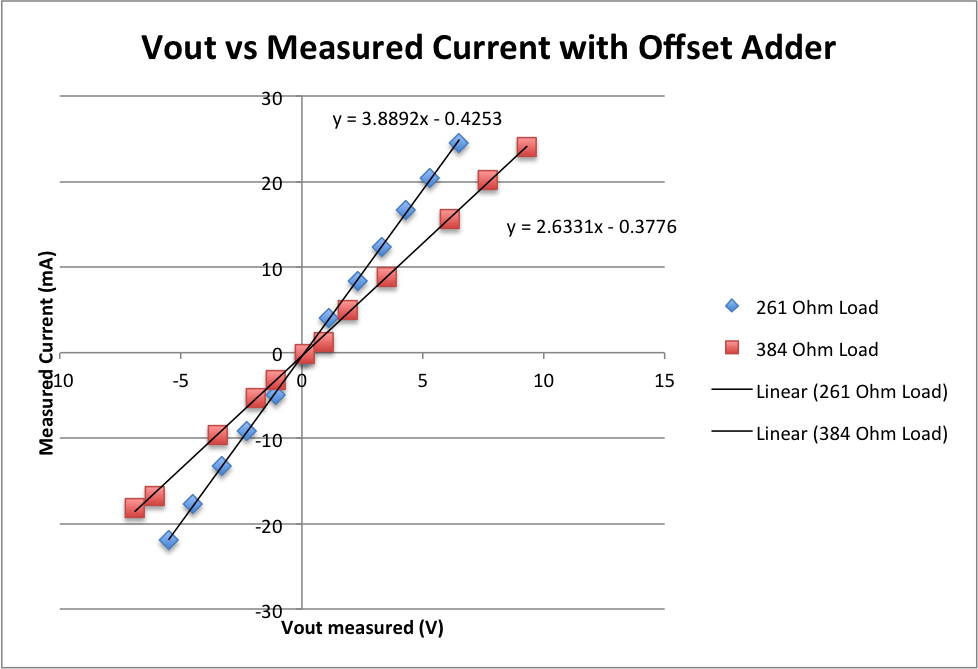
\includegraphics[scale = 0.6]{3_3.png}
        \caption{$V_{out}$ vs measured current via the offset adder for two different resistance values.}
        \label{fig:my_label}
    \end{figure}
    \begin{figure}[H]
        \centering
        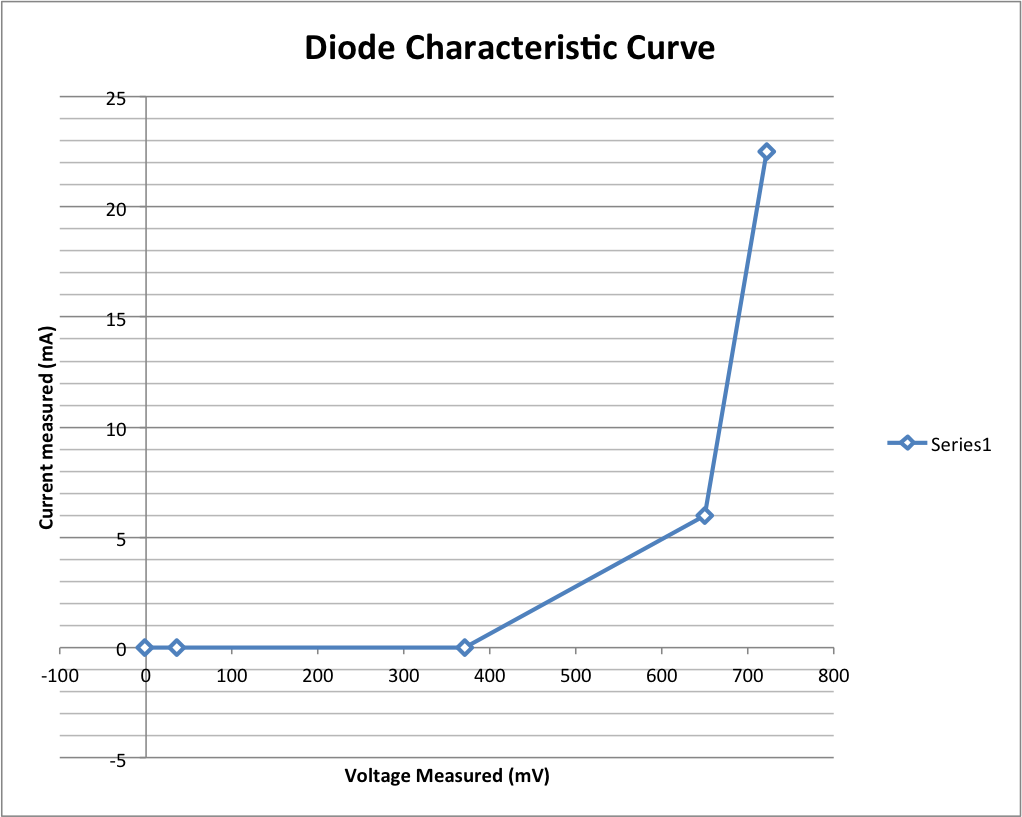
\includegraphics[scale = 0.6]{3_4a.png}
        \caption{Diode characteristic curve as discovered by offset adder analysis; linear-linear plot}
        \label{fig:my_label}
    \end{figure}
    \begin{figure}[H]
        \centering
        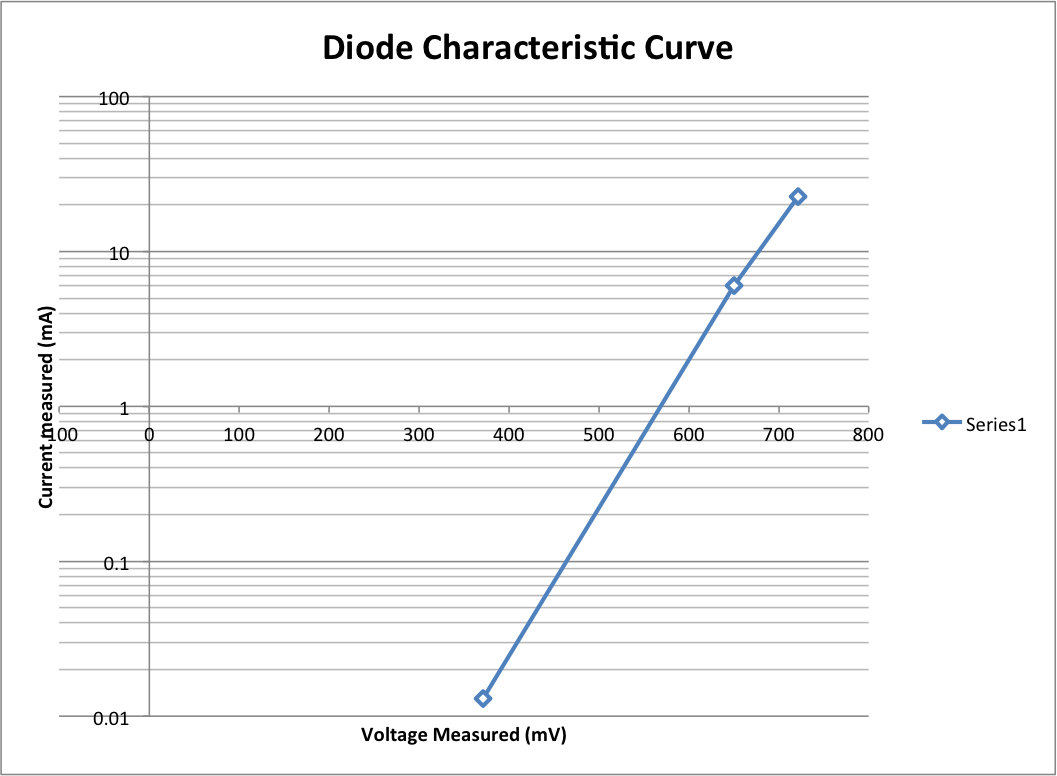
\includegraphics[scale = 0.6]{3_4b.png}
        \caption{Diode characteristic curve as discovered by offset adder analysis; log-linear plot}
        \label{fig:my_label}
    \end{figure}
    \begin{figure}[H]
        \centering
        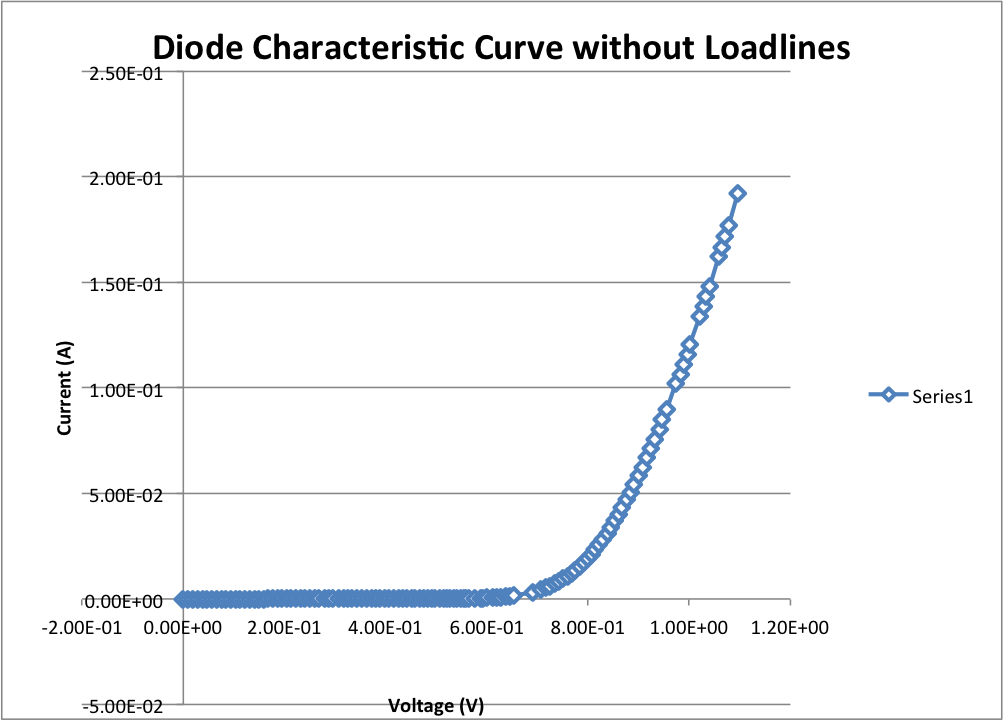
\includegraphics[scale = 0.6]{3_7.png}
        \caption{Diode characteristic curve without visualization of loadlines}
        \label{fig:my_label}
    \end{figure}
    \begin{figure}[H]
        \centering
        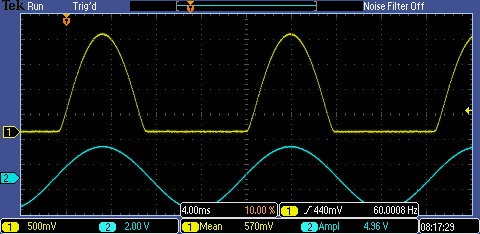
\includegraphics[scale = 0.65]{3_10.png}
        \caption{Filtered Half Wave Rectification. Channel 1 is the output signal while channel 2 is the input signal.}
        \label{fig:my_label}
    \end{figure}
    \begin{figure}[H]
        \centering
        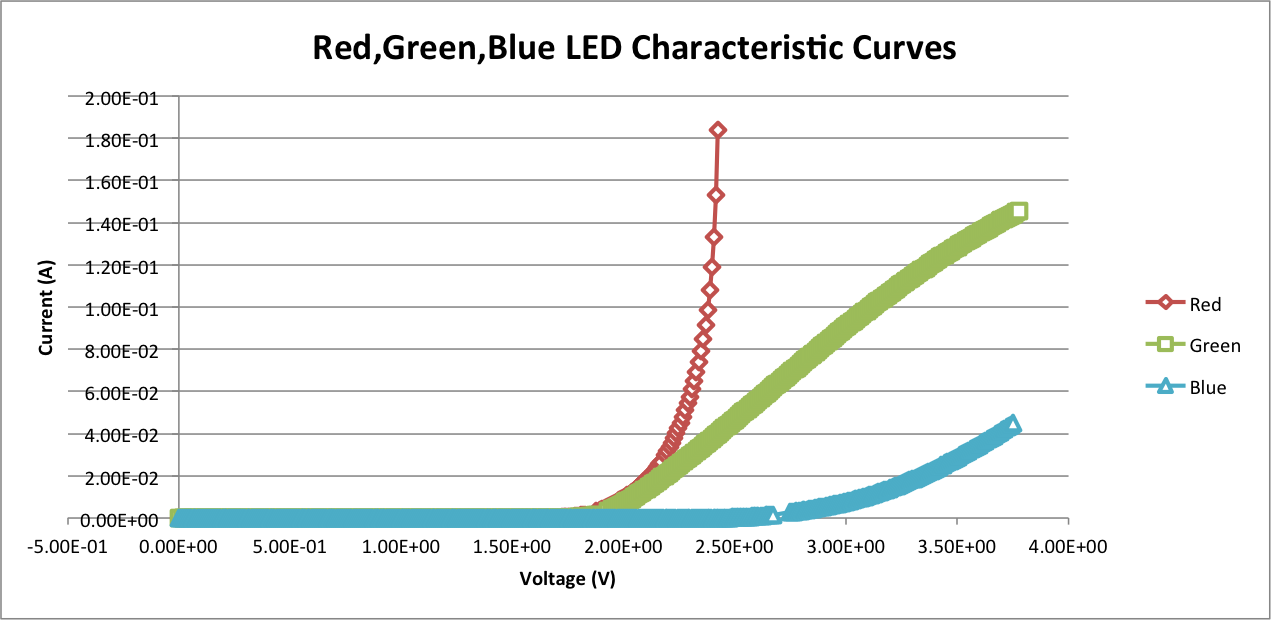
\includegraphics[scale = 0.65]{3_13.png}
        \caption{LED Characteristic Curves}
        \label{fig:my_label}
    \end{figure}
    \begin{figure}[H]
        \centering
        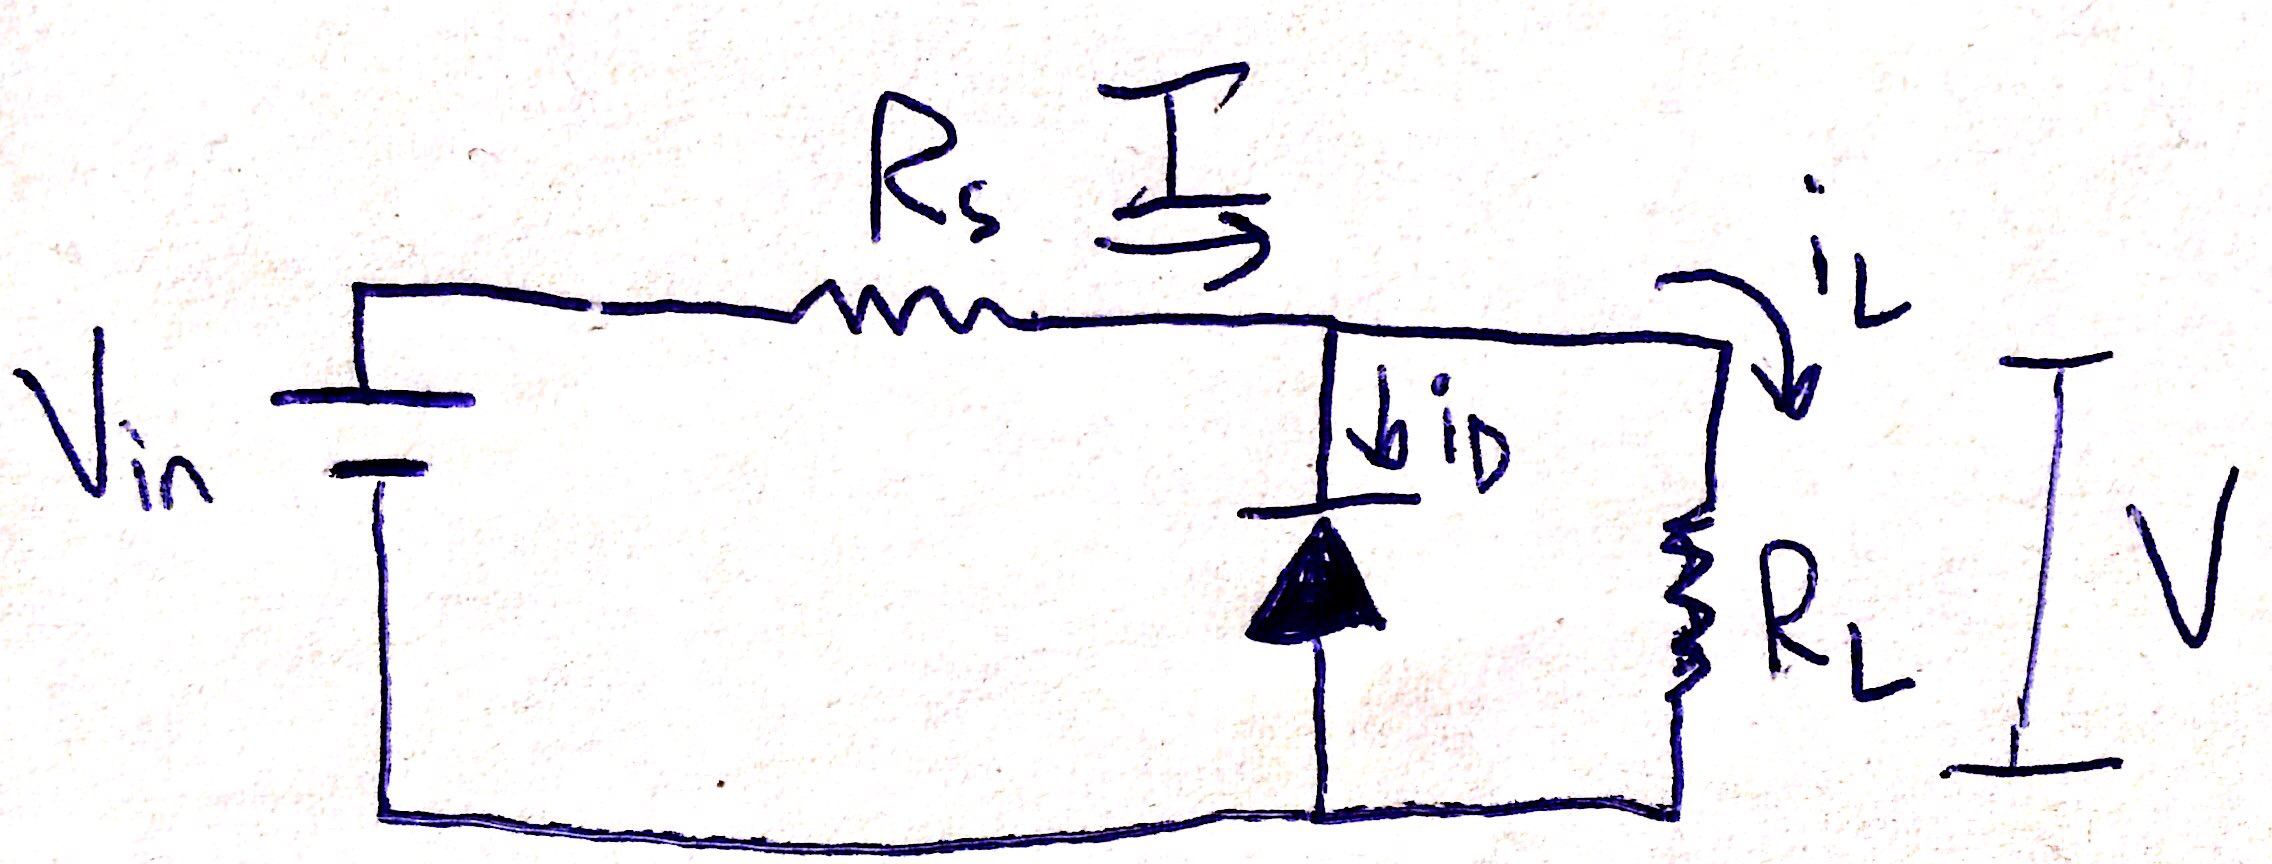
\includegraphics[scale = 0.15]{IMG_0220.JPG}
        \caption{Circuit Diagram for Zener Diode Circuit}
        \label{fig:my_label}
    \end{figure}
    \begin{figure}[H]
        \centering
        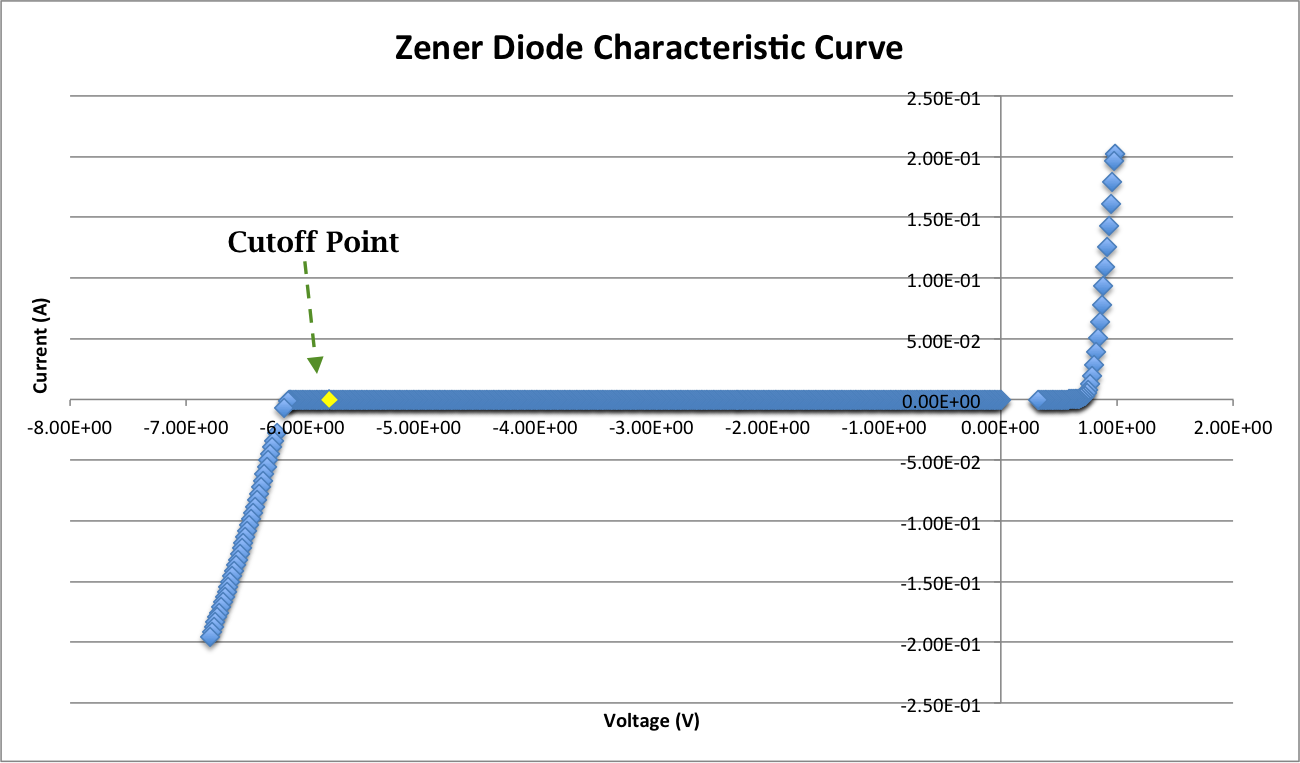
\includegraphics[scale = 0.55]{3_14b.png}
        \caption{Zener Diode Characteristic Curve}
        \label{fig:my_label}
    \end{figure}
    \begin{figure}[H]
        \centering
        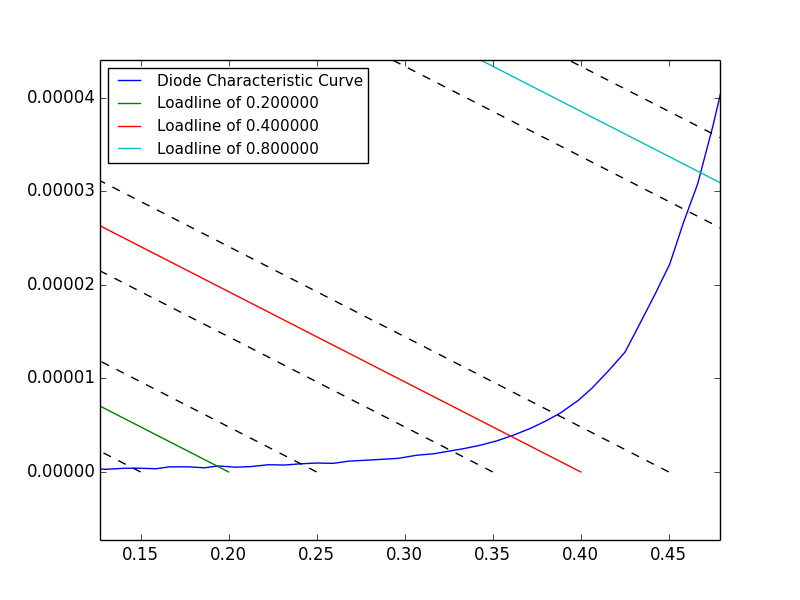
\includegraphics[scale = 0.65]{3_17.png}
        \caption{Zoomed in image of three loadlines (of offset voltages 0.2V, 0.4V, 0.8V) and their min/max amplitude loadlines (the dashed lines). The dashed lines indicate the largest and smallest value that the VDC + the VAC signal can reach. The dashed lines indicate the min/max lines of each offset voltage.}
        \label{fig:my_label}
    \end{figure}
    

\section{Signature Page}
\centering
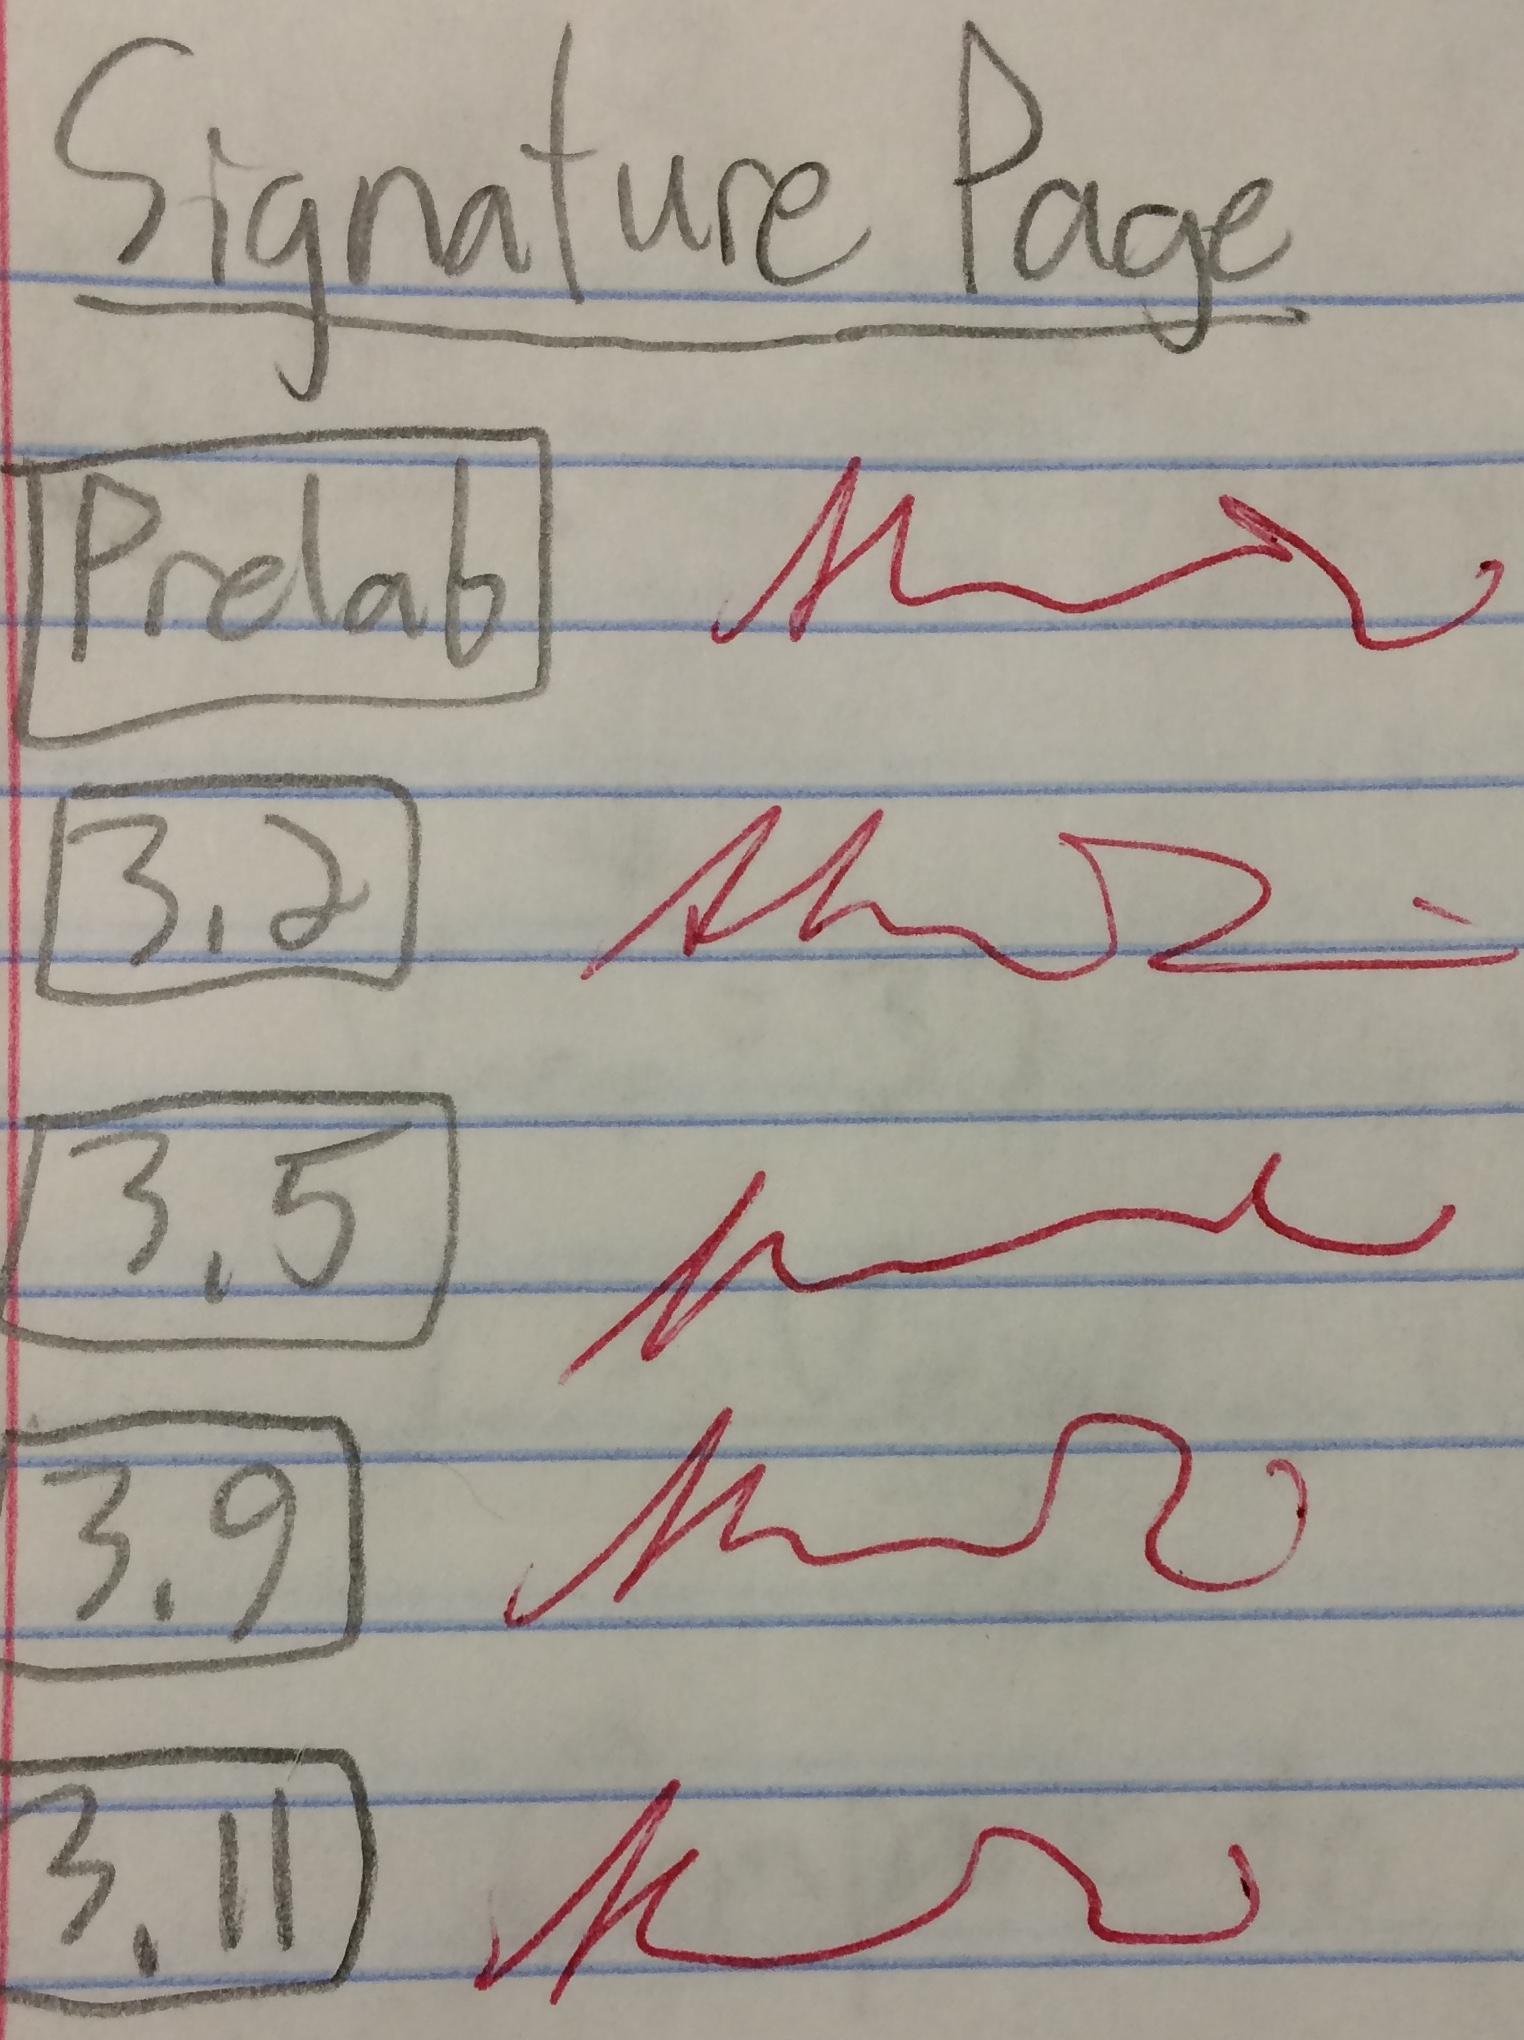
\includegraphics[scale = 0.1]{IMG_0197.jpg}


\end{document}


